\documentclass[12pt,twoside,notitlepage]{report}

\usepackage{a4}
\usepackage{parskip}
\usepackage{mathpazo}

\usepackage{verbatim}
\usepackage{algpseudocode}
\usepackage{algorithm}
\usepackage{listings}
\usepackage{minted}
\usepackage{tikz}
\usepackage{pgfplots}
\usepackage{hyperref}


\input{epsf}                            % to allow postscript inclusions
% On thor and CUS read top of file:
%     /opt/TeX/lib/texmf/tex/dvips/epsf.sty
% On CL machines read:
%     /usr/lib/tex/macros/dvips/epsf.tex



\raggedbottom                           % try to avoid widows and orphans
\sloppy
\clubpenalty1000%
\widowpenalty1000%

\addtolength{\oddsidemargin}{6mm}       % adjust margins
\addtolength{\evensidemargin}{-8mm}

\renewcommand{\baselinestretch}{1.1}    % adjust line spacing to make
                                        % more readable

\usetikzlibrary{arrows,positioning} 
\tikzset{
    %Define standard arrow tip
    >=stealth',
    %Define style for boxes
    punkt/.style={
           rectangle,
           rounded corners,
           draw=black, very thick,
           text width=6.5em,
           minimum height=2em,
           text centered},
    % Define arrow style
    pil/.style={
           ->,
           thick,
           shorten <=2pt,
           shorten >=2pt,}
}


\begin{document}

\bibliographystyle{plain}

\newcommand{\name}{Joseph Seaton}
\newcommand{\college}{Fitzwilliam College}
\newcommand{\ptitle}{Shader Compositor}

\setcounter{page}{1}
\pagenumbering{arabic}
\pagestyle{plain}

%%%%%%%%%%%%%%%%%%%%%%%%%%%%%%%%%%%%%%%%%%%%%%%%%%%%%%%%%%%%%%%%%%%%%%%%
% Title


\pagestyle{empty}

\hfill{\LARGE \bf \name ~js845}

\vspace*{60mm}
\begin{center}
\Huge
{\bf \ptitle} \\
\vspace*{5mm}
Part II Computer Science \\
\vspace*{5mm}
\college \\
\vspace*{5mm}
\today  % today's date
\end{center}

\cleardoublepage

%%%%%%%%%%%%%%%%%%%%%%%%%%%%%%%%%%%%%%%%%%%%%%%%%%%%%%%%%%%%%%%%%%%%%%%%%%%%%%
% Proforma, table of contents and list of figures



\chapter*{Proforma}

{\large
\begin{tabular}{@{\hspace{0em}}ll}
Name:               & \bf \name    \\
College:            & \bf \college \\
Project Title:      & \bf \ptitle  \\
Word Count:         & \bf About 6000 \\
Project Originator: & Christian Richardt                    \\
Supervisor:         & Christian Richardt                    \\ 
\end{tabular}
}
% detex diss.tex | tr -cd '0-9A-Za-z $\tt\backslash$n' | wc -w
\stepcounter{footnote}


\section*{Original aims of the project}
The aim of this project was to produce a novel user interface for easy composition and testing of a certain class of graphical effects known as shaders. The user interface was to be highly interactive and allow easy modification of the code for the effects themselves, the manner in which they are composed and, via graphical means, their associated parameters. Previews of these changes were to be provided as quickly as possible; therefore the project also included a number of optimisations.

\section*{Work completed}
The core of the project has been completed and works satisfactorily. Shaders can be created and a tree of shaders can be specified using JavaScript, the result of which is shown in-browser. An interface for modifying shader parameters is correctly generated for all types of parameter that have been tested, and respects some annotations. A number of optimisations have been applied, including elimination of unnecessary shader recompilation and pipeline re-generation. The project is also now capable of reusing framebuffer objects between pipeline changes where possible.

\section*{Special difficulties}
None.
 
\newpage
\section*{Declaration}

I, \name \ of \college, being a candidate for Part II of the Computer
Science Tripos, hereby declare
that this dissertation and the work described in it are my own work,
unaided except as may be specified below, and that the dissertation
does not contain material that has already been used to any substantial
extent for a comparable purpose.

\bigskip
\leftline{Signed}

\medskip
\leftline{Date }

\cleardoublepage

\tableofcontents

%%%%%%%%%%%%%%%%%%%%%%%%%%%%%%%%%%%%%%%%%%%%%%%%%%%%%%%%%%%%%%%%%%%%%%%
% now for the chapters

\cleardoublepage        % just to make sure before the page numbering
                        % is changed

%\setcounter{page}{1}
%\pagenumbering{arabic}
%\pagestyle{headings}

\chapter{Introduction}
My project provides a novel user interface for easily composing multiple graphical effects known as shaders together, in which individual shader parameters can be easily modified and the results viewed immediately. Furthermore the interface is sufficiently optimised to provide a low round-trip time between making a change and seeing the effect of this change. I have successfully implemented the core of my project, as well as a number of proposed extensions, and a few optimisations not initially proposed.

\section{Motivation}
Working with raw OpenGL is undeniably messy. OpenGL is a verbose and complicated API. When developing shaders, developers tend not to be interested in writing large amounts of OpenGL API code just to tweak shader parameters or forward the texture output of one shader to the input of another. But this is exactly what developers have to do. Given that many graphics applications are written in compiled languages like C and C++, this significantly increases the length of a development cycle. Since a large part of shader development constitutes small tweaks to (often subjectively) improve output, this is not ideal.

For students learning about shaders, OpenGL is often an intimidating and confusing mess that gets in the way of understanding a fundamentally quite simple concept.

This project aims to provide a way of developing shaders that is both useful for developers, and may be used as a tool for students learning about shaders for the first time.
\section{Brief introduction to shaders}
\label{brief}
In their modern incarnation, OpenGL shaders are quite a simple concept to understand at a high level. A shader is a simple program -- `simple' referring to certain constraints we shall ignore for now -- written in a dataflow style. Such programs take in one item of data at a time, for example a vertex, and output another item of data -- the new vertex location, or a pixel value.

In a modern OpenGL implementation, there are two commonly used types of shader (and a few more which will not be discussed). These are vertex shaders and fragment shaders. Vertex shaders operate on individual vertices, transforming the position and also attaching information such as a colour. Fragment shaders roughly speaking generate pixel values. Information can be passed from vertex shaders to fragment shaders using {\tt varying } parameters, the values of which are interpolated from those of the surrounding vertices.

\subsection{A look at some OpenGL calls}
As discussed above, the use of shaders sounds simple. However, as we can see from Listing~\ref{ugly}, a short excerpt of the OpenGL calls from an actual WebGL program\cite{reaction-diffusion}, the paraphanalia of mostly boilerplate OpenGL calls required for compiling shader programs, specifying parameters and so on can result in a very large codebase for even the simplest program.

\begin{listing}[H]
\begin{minted}{javascript}
rawData = new Uint8Array(noisepixels);
texture_noise_l = gl.createTexture();
gl.bindTexture(gl.TEXTURE_2D, texture_noise_l);
gl.pixelStorei(gl.UNPACK_ALIGNMENT, 1);
gl.texImage2D(gl.TEXTURE_2D, 0, gl.RGBA, sizeX, sizeY, 0, gl.RGBA, 
              gl.UNSIGNED_BYTE, rawData);
gl.texParameteri(gl.TEXTURE_2D, gl.TEXTURE_MIN_FILTER, gl.LINEAR);
gl.texParameteri(gl.TEXTURE_2D, gl.TEXTURE_MAG_FILTER, gl.LINEAR);
\end{minted}
\caption{Example WebGL calls}
\label{ugly}
\end{listing}

\cleardoublepage
\chapter{Preparation}

\section{Requirements analysis}
Before beginning the project, it was important to establish the general architecture. In \ref{goals} we can see a summary of the main objectives of the project. [Is this reasonable detail?]

In order to properly plan the development of the project, it was necessary to construct a graph of the dependencies between parts of the project. Priority could then be given to those parts of the project that were necessary for other parts of the core. Figure~\ref{depend} shows the general dependencies between larger parts of the project. 
\begin{table}
\label{goals}
\begin{tabular}{l | r}
Goal & Priority \\
Simple interface & High \\
Parameter detection and presentation & High \\
Pipeline generation & High \\
Pipeline rendering & High \\
Syntax highlighting & Medium \\
Optimisations & Medium \\
Annotations & Medium \\
Additional UI work & Low \\
Animation & Low \\
\end{tabular}
\caption{Main goals}
\end{table}

\begin{figure}
\label{depend}
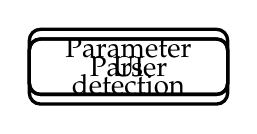
\begin{tikzpicture}[node distance=1cm, auto,]
 %nodes
 \node[punkt] (market) {Parser};
 \node[punkt] (ui) {UI};
 \node[punkt] (param) {Parameter detection};
\end{tikzpicture}
\end{figure}

\section{Preparatory learning}
\subsection{A short introduction to OpenGL}
OpenGL is a hardware, Operating System and vendor independent graphics API. It has a stateful, client-server architecture, in which the client sends commands -- OpenGL API calls -- to the server. These commands alter the current state, specifying for example that the following commands will specify a polygon. These commands enter a pipeline, a very simplified version of which is shown in [TODO diagram]. The vertex and fragment shaders discussed in Section~\ref{Brief} are contained within the per-vertex and per-fragment operation blocks respectively. Of particular concern to for this project is the final stage in this pipeline, in which fragments are rasterized and (following some other processing e.g. z-buffering) written to a framebuffer. A Framebuffer Objects or FBOs contains several buffers including a colour buffer, which may accessed as a texture by other stages.

\subsection{Background reading}

\subsubsection{OpenGL and GLSL}
Prior to beginning this project, I had very little knowledge of OpenGL barring a small amount of personal experience writing toy programs in my spare time. As such I needed to gain a better understanding of OpenGL, and some knowledge of GLSL before I could begin this project. For this purpose I obtained a copy of the famous `Red Book' \cite{redbook}. I also read through the GLSL ES specification provided by the Khronos Group \cite{glsl-spec}, which discusses the syntax of GLSL in detail.

\subsubsection{JavaScript}
While, like many people I already have some experience of JavaScript programming from web development work, I thought it would be wise to refresh myself before embarking on a more complex project such as this one. I found particularly useful {\it Eloquent Javascript }\cite{eloquent} and {\it Higher Order Programming [in JavaScript] }\cite{higher-order}, both of which are unusual among texts on JavaScript in being willing to discuss the more sophisticated functional aspects of JavaScript, and their relation to JavaScript's own unusual prototype-based object system.


\section{Development environment}
\subsection*{WebGL}
WebGL is a very recently developed API allowing web-based applications access to OpenGL ES contexts, via JavaScript \cite{webgl-spec}. It was decided that the use of web-based technologies would help lower the barrier for use of this project, and therefore shader development in general, since a user needs only visit the correct page using a modern webbrowser. Using WebGL has the added advantage of requiring less familiarisation given my prior experience with JavaScript. In \cite{webgl-spec}, we can see that WebGL uses essentially the same API as OpenGL ES for C.


\subsection*{Emacs}
Surprisingly for such an old editor, with the correct extensions Emacs is very well equipped for modern JavaScript development. While there are other editors available that could claim most or all of the features these extensions add, my previous experience with Emacs makes this a favourable choice. The extensions used add auto-completion, syntax checking, and an inline node.js (see below) console \cite{emacs-js}.

\subsection*{node.js}
node.js is a JavaScript platform built on top of Google's V8 JavaScript engine. It provides among other things, a command line interface, including a REPL (read-evaluate-print-loop). This provides a fast, light-weight way to test non-browser-bound code using traditional command line tools, can be easily interfaced with git and cron, and can easily write to files. All of this can be done without requiring messy extra code to interact with the webbrowser or server-side code to report back statistics.

\subsection*{Google Chrome}
WebGL naturally requires the use of a web browser. I have found that Google Chrome provided the most reliable WebGL implementation on my development machine, which runs Linux on an ATI HD 6850 graphics card. Since WebGL is a relatively recent development that has only recently gained browser support, WebGL can still be unstable and buggy in some circumstances even using Google Chrome. Google Chrome also includes a set of 'developer tools' including 

\subsection*{WebGL Inspector}
WebGL inspector is a Google Chrome extension intended to provide inline information on current WebGL contexts, giving easy access to state information including currently allocated textures. While this tool would be very useful for debugging, I found the tool to be insufficiently stable on my Operating System (Linux) to use reliably. This meant that most inspection of OpenGL state had to be performed manually.

\subsection{Libraries}
JavaScript as provided by web browsers is usually quite minimal in terms of provided libraries. Thanks to between-browser variation, there are also subtle (and not so subtle) differences in behaviour between browsers. It was therefore deemed pertinent to use a set of pre-existing, cross-browser libraries as discussed below. 

\subsubsection{jQuery}
jQuery is a general utility library for JavaScript, providing many helper functions not provided by browsers, and also greatly simplified DOM (Document Object Model) manipulation. In Listing~\ref{jq} we see the difference in concision with and without jQuery for some simple common tasks.

\begin{listing}[H]
\label{jq}
\begin{minted}{javascript}
// jQuery
$("a").clickfunction() {
  ...
})

// JavaScript
[].forEach.call(document.querySelectorAll("a"), function(el) {
  el.addEventListener("click", function() {
    ...
  });
});
\end{minted}
%$
\caption{Comparison of simple JavaScript tasks with and without jQuery}
\end{listing}

\subsubsection{Testing framework}
There are many unit testing frameworks available for JavaScript, of varying levels of complexity. Many of these frameworks are designed with very large projects with extensive tests in mind. For my project I considered these to be overly complicated to work with. Eventually I settled on QUnit, a very simple unit testing framework that is part of jQuery, and it's port to node.js (a fork of the original code).

\subsubsection{WebGL toolkit}
Given that OpenGL and therefore WebGL itself can be quite awkward to work with, I decided to use an existing library to abstract away some of the boilerplate code irrelevant to my project. However, there are currently many libraries available claiming to do exactly this, of varying degrees of completeness and varying levels of abstraction. Initially I settled on three.js \cite{three} on the basis of its popularity, and high rate of development. However it soon became apparent that in the level of abstraction provided by three.js actually made the task more difficult, given that interacting with FBOs was non-obvious. After some more searching I came across \textsc{glow} \cite{glow}, a toolkit specifically designed to make working with shaders simple, but otherwise providing little abstraction.

\subsubsection{Editor}
\label{cmirror}
A core aim of the project was to provide good GLSL syntax highlighting. There currently exist many web-based editors offering some degree of syntax highlighting, but I chose to use CodeMirror \cite{codemirror}, given its active development, and the presence of a modular way to add support for highlighting new grammars. 

\subsubsection{jQuery UI}
jQuery UI is a User Interface library built on top of jQuery. It provides a number of common, basic widgets including a simple tabbing interface. Using a pre-existing library is especially useful for User Interface work in JavaScript, since widgets will have been tested against multiple browsers, a time consuming and tricky process.

\subsection{Version control and backup strategy}
All project files, including the dissertation, were placed under git version control. Git is a distributed version control system, thus it was possible to maintain multiple complete copies of the repository in different locations. Git was then configured to push to multiple remote repositories in different locations: an external harddrive, my PWF account, my SRCF account, my web hosting account, and GitHub. While this could be considered excessive, the use of SSH keys meant that post-setup, this required no extra effort on my part. Since I am conscious that git is capable of history rewriting, I also configured a regular cron job to make regular compressed backups of my current repository using git bundle.

\section{Software development process}
WebGL is still quite a new technology, and as such the libraries surrounding it are not yet mature. Given that I was also not overly familiar with OpenGL at the beginning of the project, I deemed it sensible to apply an iterative software development model, to allow the requirements to be updated after prototyping. 

I decided to use an evolutionary software development model. This model employs rapid prototyping, enabling fast experimentation and evaluation of the feasibility of a given route. The model also incorporates feedback from development into the specification.

Test-driven development was also employed for some parts of the project, most prominently the parser. The use of unit testing enables early, automated detection of regressions, making it easy to spot bugs that might otherwise go unnoticed. Git pre-commit hooks were used to enforce running tests regularly. [TODO pic that isn't obviously nicked]


\cleardoublepage
\chapter{Implementation}
The project consists of the following parts:
\subsection*{Parser}
The parser extracts relevant parameters from a given shader, and their associated types, precisions and arity. Using annotations extra information for the User Interface is also extracted.
\subsection*{Pipeline specification}
The user-specified shader tree [TODO use shader tree rather than pipeline more] is extracted and converted into a usable format, with dummy objects being extended with actual shader programs.
\subsection*{Parameter UI generation}
An appropriate user interface for specifying parameters for each shader instance in the shader tree is generated based on the pipeline specification and the shader parameters extracted by the parser.
\subsection*{Pipeline generation}
A list of shaders is generated from the shader tree such that the shaders can be rendered in sequence. Actual \textsc{glow} shader objects are created. FBOs are assigned to shaders as necessary.
\subsection*{Rendering}
Render the actual pipeline, resulting in a preview image in the UI.
\subsection*{User Interface}
Connects the above stages together in an event-driven manner, and allows the user to actually input shaders and their connections and parameters. Provides feedback for errors.

\section{Parser}
The main job of the parser is to take a shader program, and provide an array of parameter names and their corresponding data types, which must be supplied to a shader program for it to run. For each parameter, the parser returns an object specifying:
\begin{itemize}
  \item A parameter qualifier: we are primarily concerned with {\tt uniform } parameters since these are exposed to the user
  \item The type: this may be a fundamental type like {\tt int} or a structure, in which case another parameter object is given 
  \item The precision: unused, but could provide error information
  \item Arity: if the parameter is an array, the size of the array
  \item Range: range annotation if present
  \item Colour: presence of a colour annotation
\end{itemize}
All of these other than the type may be left unspecified. The parser may also return information for the syntax highlighter. Since WebGL is based on a very specific version of OpenGL, OpenGL ES 2.0, the parser only needs to support GLSL ES 1.0.17 \cite{glsl-spec}\cite{webgl-spec}. This simplifies the construction of the parser, since we need not worry about different GLSL versions.

Since GLSL's is (mostly) LALR, it was deemed sensible to use a parser generator rather than expend  effort writing a parser by hand. Initially I chose to use JS/CC \cite{js-cc}, since it seemed well-documented and quite popular. However, once I had used it to generate an appropriate parser for GLSL, it quickly became apparent that the parser was insufficiently fast to use for such a complicated grammar. In fact, I was unable to obtain any timing for the parser, as under Google Chrome, even with the simplest inputs it would fail to produce any output before Chrome itself decided to kill the process. While it may have been possible to obtain timing information, this was clearly too slow to be of any value. I then found Jison \cite{jison}, a JavaScript port of Bison. This was able to parse even quite complicated input in a reasonable amount of time, as is discussed in my evaluation.

\subsubsection{Grammar conversion}
The grammar for GLSL is provided for GLSL ES in the specification \cite{glsl-spec}, in BNF form. Since Jison's specification language is roughly based on BNF, the conversion is mostly straightforward as we can see in Listing~\ref{grammar-rules}. The additional annotations between curly braces are constructing parameter type objects to be passed upwards. Token specification is likewise mostly straightforward, with the exception of struct related tokens as discussed below, and integer / floating point literals which must be represented via regular expressions. Care must also be taken with the ordering of token definitions, in particular the IDENTIFIER token is capable of capturing most keywords and must be placed after them.
\begin{listing}
\label{grammar-rules}
\begin{minted}[mathescape]{javascript}
//BNF form from specification
type_specifier:
        type_specifier_no_prec
        precision_qualifier type_specifier_no_prec

//Jison version
type_specifier:
        type_specifier_no_prec { 
          $$ = {type:$1}; 
        }
        | precision_qualifier type_specifier_no_prec { 
          $$ = {type:$2,prec:$1}; 
        }
	;
\end{minted}
%$
\caption{GLSL grammar rules}
\end{listing}

\subsubsection{Preprocessor}
GLSL contains a preprocessor language much like that used in C. It is very restricted and mostly only allows a few simple substitutions and if/else statements. It is often used to make GLSL version-based decisions, but since WebGL currently only supports one version it is not often used in WebGL programs. Implementation would require a simple initial pass over the shader code before forwarding it to the main parser. However this was dropped for time reasons [TODO: if there's time this is easy].

\subsubsection{Annotations}
In addition to parsing raw GLSL, the parser was intended to be able to detect additional annotations to parameters, providing extra information for the parameter UI, for example the range of values taken by a parameter, or whether to provide a colour picking interface. In order to keep compatiability with GLSL, it was decided to provide these annotations via comments, as we can see in Listing~\ref{unannotated}. This is acheived by way of a preprocessor that translates GLSL into annotated GLSL, an example of which we can see in Listing~\ref{annotated}. Since the syntax of these annotations is quite simple, this can be done using regular expressions. This annotated GLSL can then be passed to the parser, the grammar of which is modified to accept these annotations. An example of the rule changes can be seen in [REF TODO broken].

\begin{listing}
\begin{minted}{glsl}
uniform highp int x; //range 0,100
\end{minted}
\caption{Simple annotated GLSL parameter\label{unannotated}}
\end{listing}

\begin{listing}
\begin{minted}{glsl}
//GLSL
uniform highp float y; //range 0,100

//Annotated GLSL
uniform highp float y RANGE 0,100;
\end{minted}
\caption{Transformation to annotated GLSL\label{annotated}}
\end{listing}

\subsubsection{Struct parsing}
\label{struct-parse}
The GLSL Specification \cite{glsl-spec} allows a shader program to define and use new types of structures. These structures behave in essentially the same way as structs in C, subject to certain restrictions. Structure names and field names are subject to the same restrictions as normal identifiers. This makes parsing GLSL as parsed by e.g. Google Chrome technically context-sensitive. However, the parser used, Jison, only supports LALR grammars.

The grammar as provided in the specification introduces extra tokens for structure and field names, ignoring the context sensitivity. Therefore by way of an initial, straightforward implementation of struct parsing, I chose to make the parser simply append new structure/field names to the appropriate part of the matching logic of the lexer. While this will fail to parse shaders that use e.g. some field name as the name of a variable, or more likely, some field name as a struct name, it was deemed to be sufficient for this project.

\section{Pipeline specification}
The purpose of the pipeline specification stage is to take input from the user specifying the shaders to be used, and the connections between them - that is, when a shader uses the output FBO of a previous shader as an input texture.

For the actual pipeline specification, I could either develop my own simple specification language, or reuse some existing language. Since this project uses WebGL, it was decided to use JavaScript. This had the added bonus of enabling the user to specify a more dynamic pipeline that takes e.g. browser differences into account, with no extra work.

However, the objects used internally by my project are sufficiently complicated that I did not want to expose them directly to the user. Therefore, a simple environment containing methods for creating dummy shaders is created. These dummy shaders can then be converted into the internal format later.

In Listing~\ref{pipe} we see a simple example of a pipeline specification as provided by a user. This corresponds to the shader graph in Figure~\ref{pipe-graph}. The variable ``output'' is special, in that it corresponds to the highest node in the 'tree' and therefore the final node in the pipeline. Notice that some parameters are left blank -- these can be provided later via the parameter UI. Individual shader instances can be given names for identification within the UI, and the size of the FBO to which the shader is drawn can also be specified (with sensible defaults provided for both). Unfortunately, since JavaScript lacks a way to dynamically find the variable names within a given context, it is not possible to automatically infer shader instance names without using a JavaScript parser, which is beyond the scope of this project (and would not always be able to infer names since shader instances can be anonymous).
\begin{listing}[H]
\begin{minted}{javascript}
output = new gaussHShader("output");
gaussv = new gaussVShader();
input = new textureShader("input",{width:800,height:600});

output.img = gaussv;
gaussv.img = input;
\end{minted}
\caption{Example pipeline specification\label{pipe}}
\end{listing}

\begin{figure}

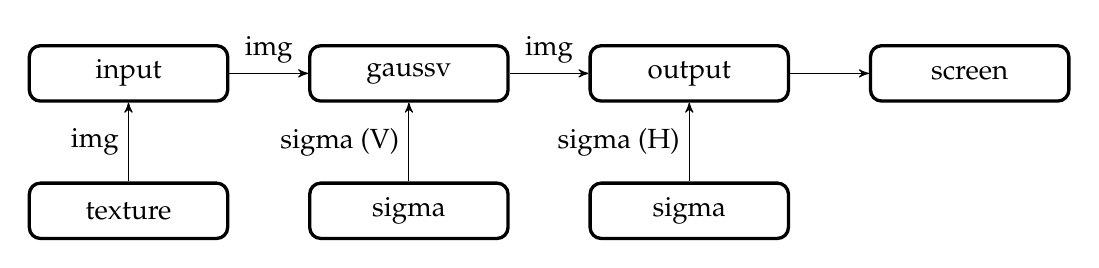
\begin{tikzpicture}[->,node distance=1cm, auto,]
\node[punkt] (input) {input};
\node[punkt, below=of input] (texture) {texture};
%edge[pil,->] (input.south);
\node[punkt, right=of input] (gaussv) {gaussv};
%edge[pil,<-] (input.east);
\node[punkt, right=of gaussv] (output) {output};
%edge[pil,<-] (gaussv.east);
\node[punkt, right=of output] (screen) {screen};
%edge[pil,<-] (output.east);

\node[punkt, below=of gaussv] (gaussv-sigma) {sigma};
%edge[pil] (gaussv.south);
\node[punkt, below=of output] (output-sigma) {sigma};
%edge[pil] (output.south);

\path   (texture) edge              node {img} (input)
        (input)   edge              node {img} (gaussv)
        (gaussv)  edge              node {img} (output)
        (output)  edge              node {} (screen)
 (gaussv-sigma)   edge              node {sigma (V)} (gaussv)
 (output-sigma)   edge              node {sigma (H)} (output);

\end{tikzpicture}
\caption{Shader graph\label{pipe-graph}}
\end{figure}

\section{Parameter UI generation}
\label{ui-params}
This stage takes a tree of dummy shaders, and creates the appropriate HTML user interface. For each parameter of the shader which needs specifying -- that is, is of type {\tt uniform} and is not already specified -- it produces an appropriate set of input elements. For each parameter a label based upon either the provided name or a hopefully informative generated name is generated, along with a type-specific label and widget.

In the initial implementation, the appropriate shader values would be updated when a new render was requested. However this is inefficient, and makes the user interface less responsive. Later implementations therefore use a different method: each input element has associated event listeners that will update the value within the shader, and correctly invalidate the \textsc{glow} cache and request the preview be re-rendered.

While simple text boxes provide complete control over the parameters, for certain types of parameter more useful widgets can be provided. The most obvious example is for {\tt vec3 } and {\tt vec4 } (vectors of length 3 and for) parameters, which are often used to specify colours. For such parameters, I constructed a colour picking widget based on the web colour picker by Stefan Petre \cite{color}, as can be seen in [TODO].

\subsection{Struct handling}
Since \textsc{glow} expects structure parameters to be specified by ordinary JavaScript objects, which are also used to specify parameters, structs can be easily and simply handled by recursing on the parameter generation function. While for languages like C, this could produce an infinite loop if the structure references itself, GLSL does not permit this. However, the parser will not reject such a self-referential structure definition, which would cause infinite recursion. This is avoided using a counter set to a sufficiently large value that no valid GLSL program could reach it. This is possible since GLSL programs are required to compile to a sufficiently small amount of instructions, due to the limitations of stream processors.

\section{Pipeline generation}
\subsection*{Pipeline linearisation}
At this stage in the process, we have essentially a Directed, Acyclic Graph (DAG) of shader instances, with connections representing dependencies between instances -- that is, instances that write to textures that will be read by other instances. In order to actually render the DAG, we must linearise such that the node labeled output is last. This is the primary task of the pipeline generation stage, namely converting the shader DAG into a list. This can be acheived using a topological sort. Initially the algorithm decribed by Cormen et al \cite{topsort} was used. The algorithm is shown in Listing~\ref{simpletopological}.
\begin{algorithm}
\label{simpletopological}
\begin{algorithmic}
\State $L \gets $ Empty list that will contain the sorted nodes
\State $S \gets $ Set of all nodes with no outgoing edges
\ForAll{node n in S}
    visit(n)
\EndFor 
\Function{visit}{node}
    \If{n has not been visited yet}
        mark n as visited
        \ForAll{node m with an edge from m to n}
            visit(m)
        \EndFor
        add n to L
    \EndIf
\EndFunction
\end{algorithmic}
\end{algorithm}
However, the algorithm shown in Listing~\ref{simpletopological} cannot detect when the graph contains a loop. This situation will only occur if the user inputs an invalid shader graph -- in such a case, the program should produce an error.

\subsection*{Pipeline initialisation}
\label{pipe-init}
In this stage, each shader object in the pipeline must be assigned an actual \textsc{glow} shader. This is the object that contains the actual compiled shader that will be called at rendertime. Initially, this was done in the most straightforward manner possible, by simply iterating through the pipeline and generating new \textsc{glow} objects after any modification. All parameter values would be retrieved from the UI at this point. This required the user to manually request the pipeline be updated before rendering. 

Recreating \textsc{glow} objects and reading in all parameter values after a single parameter change is very inefficient, especially since this process would run after each individual parameter change. Therefore this stage was later modified such that changing parameters would not require a complete update -- \textsc{glow} objects are created before the Parameter UI Generation stage, with dummy parameter values, and pipeline initialisation is only run after a change to the pipeline (as discussed in Section~\ref{opt}.

\section{Rendering}
The rendering process itself is kept simple, since we try to offload as much work as possible to other stages. This is important for later extensions involving animation, where we want the render loop to run as quickly as possible. The render loop simply iterates through the shader pipeline list, binding the FBO associated with each shader, rendering the shader, and then unbinding the FBO. The FBO binding is skipped for the final shader, which is instead rendered to the preview context. While the initial render function cleared the \textsc{glow} cache at the start of each call, we can avoid this as discussed under Section~\ref{glow-cache}.

\section{Optimisation}
\label{opt}
As stated in the introduction, one of the main aims of this project is to make the User Interface as interactive as possible. To be more specific, the delay between making some change and seeing the effect of this change should be as short as possible. Since changes on this timescale will usually be quite small, for example changing a single parameter, or modifying a single shader, by reusing existing state where possible this delay can be significantly reduced.

\subsection{\textsc{glow} early initialization}
As discussed in Section~\ref{ui-params} and Section~\ref{pipe-init}, in the initial implementation all stages following Parameter UI Generation must be called, at the users request, following each change to a parameter. This includes a step in which every parameter in the UI is updated, initialisation of \textsc{glow} shader objects, and pipeline linearisation. This is obviously suboptimal, both since all parameters must be updated and redundant steps be re-run, and since the user is required to request re-rendering, which reduces the level of interactivity.

The solution to this problem is briefly mentioned in Section~\ref{pipe-init}. Rather than creating \textsc{glow} objects -- and therefore incurring compilation overhead -- after all parameters have been specified, we substitute dummy parameters of the appropriate type, and create the \textsc{glow} objects during shader tree creation (that is, during the pipeline specification stage). Dummy parameters are obtained by modifying the parameter UI generation stage to generate a dummy value for each parameter as well as the actual UI. Parameter changes now generate events which update the relevant \textsc{glow} object's parameters, and request a new render. The entire pipeline initialisation stage can now be skipped. Updates also invalidate the relevant \textsc{glow} cache as discussed below.

\subsection{Modified shader detection}
\label{msd}
The implementation as discussed above performs the entire shader parsing through pipeline initialization process, throwing away all previous data, whenever a shader program is modified. Since only one shader program can be modified at once, this is sub-optimal. This is particularly important since we would like to be able to render a new preview of the pipeline output as quickly as possible. The most obvious optimisation here is to only update shader instances in the pipeline that use the modified shader. This is achieved by tagging shader instances with the name of their shader. Shader update calls then only need to attach new \textsc{glow} shaders to the appropriate shaders, using their existing parameters. Note that this is only applicable if the required shader parameters have not been added to or changed, since all parameters must be specified. In this case the old behaviour can be falled back on.

\subsection{Parameter value propagation}
Some of the advantages in interactivity introduced by the optimisations made in Section~\ref{msd} will be useless, since parameters specified for the modified shader will be lost, and will need to be re-entered by the user. However we cannot simply reuse the previous shader parameters since the parameters taken by said shader may have changed. The set of parameters for the modified shader must first be compared to the new required parameters, and dummy parameters generated where appropriate and any extra parameters must be discarded (these extra parameters are ignored, and we could try to keep these parameters in case they are used in the future [TODO: if I get really bored]). 

\subsection{\textsc{glow} cache}
\label{glow-cache}
For efficiency reasons, \textsc{glow} itself tries to cache as much as possible in GPU-accessible memory. In particular, parameter values are cached and updates to parameters must respect this and invalidate the cache before the next render call. In the initial implementation, the \textsc{glow} cache was cleared at the start of each render call. This is inefficient, and was soon modified such that the \textsc{glow} cache was only cleared after parameter changes and pipeline changes. However, this is still not particularly efficient, as these gains are mostly only noticable during animation. 
[TODO: can do better?]

\subsection{FBO reuse}
In the initial implementation, FBOs are simply discarded and new FBOs are allocated after each pipeline change. This is time consuming and could be avoided. However, since FBOs come in different sizes, we cannot naively allocate some 'pool' of available FBOs. This is achieved by simply keeping separate pools of already allocated FBOs for each size of FBO that has been used in the past. Shader updates using the event-based system described above can reuse the existing FBO for each instance, this is an additional benefit of the optimisations discussed.

\section{User Interface}
\subsection{Editor}
As discussed in \ref{cmirror}, I chose to use the CodeMirror text editor to provide GLSL syntax highlighting to users. While CodeMirror does not provide GLSL highlighting, it does provide a general, 'C-like' highlighting mode, and simple hooks for custom parsers. Initially, I based my syntax highlighting on the 'C-like' mode provided. This was a simple matter of providing the correct keywords. However, this only provides simple highlighting. Given that each shader is parsed anyway, it would seem sensible to modify the parser used for parameter extraction to also provide syntax highlighting information. [TODO: actually do this]

\subsection{Layout}
The initial layout of the UI was straightforward, consisting of a pair of text editors for each shader program, a text editor for the pipeline and parameter specification, a sequence of control buttons and a preview box. [TODO picture]. While this layout was spartan and not user friendly, it was sufficient for initial testing, and allowed for easy debugging of separate stages.
\subsection{Improved Layout}
The layout described above suffers from a number of usability problems. Firstly, the UI does not fit at all on an average-sized screen. This requires the user to be constantly scrolling to use it, adding a delay between the user making a change, and seeing its effect. Secondly, the control buttons are unintuitive, and the need for the user to use them whenever they wish to see the effect of a change further increases the expected length of a user's development cycle. A new layout was designed, with inspiration taken from the typical construction of IDEs, where tiling is employed to maximize screen usage. From [TODO another picture] we can see the improved layout. Shader programs occupy the top left side of the screen, and can be switched between by clicking on the shader's name. The right hand side of the screen is occupied by the parameter specification UI at the bottom, and the preview at the top. The control buttons have been eliminated entirely using the hooks developed in Section~\ref{opt}. Compared to the old layout, this provides:
\begin{itemize}
\item Minimal scrolling -- shaders/pipeline specification/parameters can be changed without having to scroll to see the result
\item Improved interactivity -- updated render provided as soon as possible, rather than on request
\item Improved usability -- no confusing buttons to press requiring knowledge of internal program workings 
\item Error feedback -- introduction of an error popup means users are informed of errors, but screen space is not wasted otherwise
\end{itemize}
\cleardoublepage
\chapter{Evaluation}
Evaluation of this project chiefly consists of two parts, correctness and performance. Correctness evaluation is intended to demonstrate correct functioning of the core project. Performance evaluation provides an analysis of the effect in terms of both performance and resource usage of some of the optimisations.

\section{Parser correctness}
In order to assist with development of the parser, and in particular to assist in regression testing, a test harness was developed for the testing the correctness of parameters returned by the parser. Since the parser does not access any browser-specific APIs, it was possible to perform this testing in a simple, automated way on the command line. Each test is specified by a shader program, and the result that should be returned by the parser -- the parameters and their associated information, any struct definitions, and whether the parser should fail to parse it and raise an exception, in the case of an invalid program. Parser output for each test specification is then compared against the actual output for a set of tests. These include correctly throwing/not raising an exception, returning the correct parameter names/a correct subset of the parameter names, all/some of the correct parameter types, the correct struct definitions, and so on. An additional script was written to perform these tests over all git revisions. 

In Section~\ref{parser-git} we see a graph showing the percentage of tests correctly completed, from the first revision including a parser. The notable jumps in tests passed correspond to implementation of the currently used parameter format, scoping corrections (i.e. discarding parameters hidden within functions) and structure support. Not all tests are passed at the final version -- these tests are those that contain structure definitions and variables with the same name, the parsing of which is not possible with my current parser, as discussed in Section~\ref{struct-parse}. Also tests that use preprocessor commands will fail since a preprocessor was not implemented.[TODO more tests]

\begin{figure}
\label{parser-git}
\begin{tikzpicture}
\begin{axis}[xlabel={git revision},ylabel={tests passed}]
\addplot file {parser.data};
\end{axis}
\end{tikzpicture}
\end{figure}

\section{Pipeline correctness}
[TODO: don't really have this, getting output is a real pain. Possibly construct a set of demonstrations that clearly work? Good excuse to make pretty pictures.]
In order to demonstrate visually correct shader pipeline output, a small number of example pipelines were constructed. This was achieved by taking a sample of simple WebGL example programs found online, and modifying them to work within my project. Output from the modified versions could then be compared with the originals. Ideal example programs would use a few different shaders connected together to produce a single visual effect. Below we can see samples of the output of the original programs alongside my reimplementations.

\section{Performance}
\subsubsection{Effect of modified shader detection}
In Section~\ref{opt}, we discussed the modification of the pipeline initialization process to avoid unnecessary shader re-parsing, compilation, and pipeline generation after modification of a shader. In order to compare the performance of the updating procedure before and after these optimisations were introduced, a custom test harness was developed. Since the existing test harnesses for JavaScript that provide performance testing are mostly quite heavyweight, being intended for large-scale website testing, I implemented this from scratch.

Each test specification consists of a set of shaders, and a shader tree specification in which all necessary parameters are specified. Once a shader pipeline has been generated for a given specification, a shader update event is generated for a particular shader, and its completion timed. This is repeated 10 times to obtain an average and range. Similarly the completion of a complete re-generation of the shader pipeline is timed 10 times. This is repeated for each shader in the test specification. From [TODO graph] we can see the result of these tests for a particular test specification.

\subsection{Effect of FBO reuse}
Also in Section~\ref{opt}, we discussed the modification of the pipeline initialization process to reuse FBOs where possible. While the main motivation for this is to avoid allocating textures unnecessarily, this has possible speed benefits. [TODO graph]

\section{Texture usage}
In Section~\ref{opt}, we discussed 

\cleardoublepage
\chapter{Conclusion}

\section{Main Results}
The project has been successful. The core of the project has been completed and functions correctly, and with the addition of the various optimisations and extensions, is sufficiently interactive to be useful. I have made the project source code availabe to others via GitHub, and I hope that it will prove useful. In Table~\ref{core_t} we can see that the core critera were completed, and from Table~\ref{ext_t} we can see that a significant number of the extensions were completed. In addition, a number of optimisations were made not listed in the table below.

\begin{table}
\begin{tabular}{p{9cm} | r}
Criterion & Successful? \\
Interface to construct shaders, specify connections between shaders & Yes \\
Detection of parameters of set of shaders, parameters presented to the user somehow & Yes \\
Sample scene output for single shader & Yes \\
Demonstration of correct composition (with sample scene output) for various shaders with pipeline specifications & No [SEE EVAL]\\
Provide basic syntax highlighting of GLSL in interface & Yes \\
\end{tabular}
\label{core_t}
\caption{Core Criteria}
\end{table}
\begin{table}
\begin{tabular}{p{9cm} | r}
Criterion & Successful? \\
Reuse of FBOs in shader pipeline & Yes \\
Automatic unification of identical textures & No \footnotemark[1] \\
Splitting shared code off into separate shaders & No \footnotemark[2] \\
Avoiding recompiling shaders unnecessarily & Yes \\
Presentation of sliders with range detected from range annotations in shaders & Yes[TODO broken]\\
Some facility for animation & No \\
Shader and/or scene test suite & No \\
\end{tabular}
\footnotetext[1]{This is done automatically anyway }
\footnotetext[2]{This feature would require a lot of work for questionable benefits, and was dropped}
\label{ext_t}
\caption{Extensions}
\end{table}
\section{Lessons learned}
The combination of WebGL and Linux is still a little unstable at times, and as such I would be apprehensive about relying so much on a very recent technology for future projects.

While I was initially apprehensive about using JavaScript given it's reputation as an ugly language to work with, I was pleasantly surprised by it's novel object model and quite functional underpinnings. Particularly useful was the ability to apply a class constructor to an already existing object [TODO why].

\section{Further work}
As this project was only partially focused on the development of a user interface, the current UI is fairly basic. Further work could be done to make the UI more usable, and possibly to conduct a user study to test its effectiveness. More sophisticated widgets and better error feedback would be a good start. The extensions listed in Table~\ref{ext_t} were dropped for time reasons, but could also be incorporated with not too much additional effort.

Both the specification and implementation of WebGL have changed significantly since their first proposal, and I expect them to continue to do so for some time yet. As such further work may be necessary in the future as these change. Of particular note is the current lack of multiple render targets in current implementations \cite{webgl-future}. If in the future implementations begin to support multiple render targets, adding support for these to my project will be a moderately non-trivial task.

\cleardoublepage

%%%%%%%%%%%%%%%%%%%%%%%%%%%%%%%%%%%%%%%%%%%%%%%%%%%%%%%%%%%%%%%%%%%%%
% the bibliography

\addcontentsline{toc}{chapter}{Bibliography}
\bibliography{refs}
\cleardoublepage

%%%%%%%%%%%%%%%%%%%%%%%%%%%%%%%%%%%%%%%%%%%%%%%%%%%%%%%%%%%%%%%%%%%%%
% the appendices
\appendix

%\chapter{Latex source}

%\section{diss.tex}
%{\scriptsize\verbatiminput{diss.tex}}

%\section{proposal.tex}
%{\scriptsize\verbatiminput{proposal.tex}}

%\section{propbody.tex}
%{\scriptsize\verbatiminput{propbody.tex}}



%\cleardoublepage

%\chapter{Makefile}

%\section{\label{makefile}Makefile}
%{\scriptsize\verbatiminput{makefile.txt}}

%\section{refs.bib}
%{\scriptsize\verbatiminput{refs.bib}}


\cleardoublepage

\chapter{Project Proposal}

%
% Draft #1 (final?)

\vfil

\centerline{\Large Part II Computer Science Project Proposal}
\vspace{0.4in}
\centerline{\Large Shader Compositor }
\vspace{0.4in}
\centerline{\large Joseph Seaton, Fitzwilliam College}
\vspace{0.3in}
\centerline{\large Originator: Christian Richardt}
\vspace{0.3in}
\centerline{\large 21 November 2000}

\vfil

\subsection*{Special Resources Required}

\vspace{0.2in}

\noindent
{\bf Project Supervisor:} Christian Richardt
\vspace{0.2in}

\noindent
{\bf Director of Studies:} Dr R. Harle
\vspace{0.2in}
\noindent
 
\noindent
{\bf Project Overseers:} [TODO]

\vfil
\pagebreak

% Main document

\section*{Introduction}
Designing shaders can be laborious work, involving endless back and forth between tweaking the
code (often minor visual tweaks) and examining the visual output. While programs exist to provide
previews of individual shaders, modern software, especially for computer game engines, often
involves multiple shaders chained together, and little software exists to aid shader writers in testing
such shader pipelines. Furthermore for beginners, the initial process of learning of how to use
shaders is complicated by this extra legwork to compose shaders. The aim of this project is to
alleviate these problems to some degree.

\subsection*{Aside on Shaders}
A 'shader' is a piece of code that runs directly on a GPU. Shaders work on the data flow model, in
that once the code is set up, many data may be fed through it. In OpenGL, which this project will
focus on, such shaders are divided into a number of types. The two types considered here are vertex
shaders and fragment shaders although there are others including geometry shaders which could be
considered as an extension. Vertex shaders operate on a vertex, and its associated data, performing
such operations as transforming a vertex to the screen coordinates. Fragment shaders
(approximately speaking) operate on individual pixels, and are often used for operations such as
texturing a model. Vertex shaders may pass information to fragment shaders, and the underlying
program using the shaders may pass information to both.

\subsection*{The Project}
This project intends to provide an interface to allow a user to create a set of shaders, written in a
slightly annotated version of GLSL. The attributes of these shaders will be detected, along with the
type of each attribute, and, given a specification of how to connect these attributes (provided either
via a GUI or a simple language), a pipeline of these shaders will be constructed.
It should be noted that the construction of said pipeline will require a number of stages, namely
construction of a simple GLSL parser, generation of a DAG of shaders, linearisation of said DAG,
and finally application of this DAG to FrameBuffer Objects for offscreen rendering, finishing in
some rendered model. Since FBOs can be reused, an efficient mapping is non-trivial. Furthermore,
there is room for optimisation of this DAG – consider unification of identical textures, or extraction
of common code.
The interface should also provide some facility to allow the user to easily modify shader parameters
by e.g. selecting textures, or setting the colour of a vector. Addition of simple annotations to the
GLSL may be useful here, such as specifying the range of a vector.
Since this project is intended to be used partly as a learning tool, I propose to use WebGL, a
standard for using OpenGL (including GLSL) on the web, via JavaScript. Since WebGL is cross
platform by design and requires only a recent webbrowser to use, As WebGL is quite a new
technology, it is possible that this may turn out to be infeasible, in which case I would use Python.

\subsection*{Resources Required}
Since this project will involve OpenGL shaders, a recent graphics card supporting a recent version
of OpenGL will be required. To this end I would use my own computer with its AMD HD5450
graphics card. Depending upon the speed at which my test harness runs, I may consider upgrading
to a more powerful card such as the HD6770.

\subsection*{Starting Point}
I have some existing knowledge of OpenGL and GLSL from personal experience, but only to the
extent of small personal projects. I have a reasonable amount of experience with JavaScript having
used it in the past for web development work – but in conjunction with a server-side language.
Substance and Structure of the Project
The project involves writing software providing a user interface in which to input a set of shaders
and the connections between them and view a sample output of the generated shader pipeline on a
sample model.
Most notably to do this the project requires software to be written that given a set of shaders and a
specification of how to connect them, can parse each shader, extract its parameters, and construct
the specified pipeline.
Furthermore the user interface should provide the ability to easily vary the parameters of each
shader on the fly. This and the above comprise the core of the project.
By way of extensions, there is much scope for fleshing out the interface into a fully-featured
development tool, with such additions as example shaders, a more complete set of sample scenes,
and so on. There is also some room for optimisation of the composition process, for example the
unification of identical textures or extraction of common code between shaders.
For evaluation, in order to demonstrate correct composition, a testing framework will be written that
takes a set of semantically obvious or simple shaders and composites them in arbitrary ways and
tests whether the output matches the expected result. Also pipeline speed/memory use comparisons
of before/after the implementation of the extensions will be performed, along with comparisons of
recomplilation speed before/after optimisation (i.e. detection of modified shader). Further
comparisons include comparisons of a generated pipeline against a hand-coded shader, or a
comparison of the time complexity of a given pipeline to a JavaScript program carrying out the
same task.


\section*{Success Criteria}
The following should be achieved:
\begin{enumerate}
\item Interface to construct shaders, specify connections between shaders
\item Detection of parameters of set of shaders, parameters presented to the user somehow
\item Sample scene output for single shader
\item Demonstration of correct composition (with sample scene output) for various shaders with
pipeline specifications
\item Provide basic syntax highlighting of GLSL in interface
\end{enumerate}
Extensions:
Demonstration of some optimisations:
\begin{enumerate}
\item Reuse of FBOs in shader pipeline
\item Automatic unification of identical textures
\item Splitting shared code off into separate shaders
\item Avoiding recompiling shaders unnecessarily
\end{enumerate}
Demonstration of some additional GUI work:
\begin{enumerate}
\item Presentation of sliders with range detected from range annotations in shaders,
\item Some facility for animation (e.g. parameters that are automatically incremented)
\item Shader and/or scene test suite
\end{enumerate}

\section{Timetable and Milestones}
\subsection{Weeks 0-2: 22nd October – 11th November}
Initial reading. In particular, the OpenGL 'red book'. Setup of barebones GUI, associated libraries.
Preparation of automatic backups.
Milestone: dummy interface for single shader.
\subsection{Weeks 3-5: 12th November – 2nd December}
Construction and testing of GLSL parser. Further familiarisation with GLSL.
Milestone: ability to parse simple GLSL
\subsection{Weeks 6-8: 3rd December – 23rd December}
Write shader DAG generating code, DAG linearisation code. Initial work on application to FBOs.
Milestone: generation of linearised shader DAGs
\subsection{Weeks 9-11: 24th December – 13th January}
Complete actual pipeline – given some DAG, the project should be able to render the pipeline to a
quad. Complete interface such that the pipeline order can be specified, either via a GUI or via some
written specification. Basic parser may be sensible.
Milestone: ability to render a given shader pipeline
\subsection{Weeks 12-14: 14th January – 3rd Feburary}
Preparation of progress report. Presentation of shader parameters in GUI. Initial
work on texture unification and other optimisations. Initial work on test suite.
Milestone: Progress report prepared. Ability to vary shader parameters from the GUI. Ability to
unify some identical textures (or reduced FBO or code usage, depending on extension). Some tests
written.
\subsection{Weeks 15-17: 4th February – 24th February}
Presentation of progress report. Further testing of core functionality, expansion of test cases. Bug
fixing. Possibly initial
optimisation work.
Milestone: Progress report given. Large test suite. Lack of obvious bugs in core.
\subsection{Weeks 18-20: 25th February – 16th March}
Additional GUI work and/or optimisation. Slack time for unexpected problems. Optimisations can
be skipped if more time is needed for core work.
Milestone: Better featured GUI and/or some further optimisations.
\subsection{Weeks 21-23: 17th March – 6th April}
Begin work on dissertation. Programming work should be finished by now, although some
expansion of the test suite may be acceptable.
Milestone: complete initial sections of dissertation.
\subsection{Weeks 24-26: 7th April – 27th April}
Finish first draft of dissertation.
\subsection{Weeks 27-29: 28th April – 18th May}
Proofreading and submission.


\end{document}
